% !TEX TS-program = pdflatex
\documentclass[11pt,a4paper]{article}

% ---------- Encoding & Fonts (robust UTF-8, proper glyphs) ----------
\usepackage[utf8]{inputenc}
\usepackage[T1]{fontenc}
\usepackage{textcomp} % for \textminus with T1
% Robust Unicode mappings for pdfLaTeX:
\DeclareUnicodeCharacter{2014}{\textemdash} % — em dash
\DeclareUnicodeCharacter{2013}{\textendash} % – en dash
\DeclareUnicodeCharacter{2212}{\textminus}  % − minus

% ---------- Typography & Layout ----------
\usepackage[landscape, margin=0.5in]{geometry}
\usepackage{microtype}
\usepackage{parskip}         % space between paragraphs, no indents
\usepackage{setspace}
\usepackage{titlesec}
\usepackage{enumitem}
\usepackage{booktabs}
\usepackage{csquotes}
\emergencystretch=2em % help avoid overfull boxes for long paths

% ---------- Fonts ----------
\usepackage[scaled]{helvet}
\usepackage{newpxtext,newpxmath} % Palatino-like text+math

% ---------- Math & Algorithms ----------
\usepackage{mathtools,bm}
\usepackage{float} % for [H]
\usepackage[ruled,vlined,linesnumbered]{algorithm2e}

% Theorem environments (after newpxmath to avoid conflicts)
\newtheorem{definition}{Definition}
\newtheorem{theorem}{Theorem}
\newtheorem{remark}{Remark}

% ---------- Graphics & Figures ----------
\usepackage{xcolor}   % ensure colors are defined before TikZ/pgfplots
\usepackage{graphicx} % needed for \includegraphics and \resizebox
\usepackage{caption}
\usepackage{tikz}
\usetikzlibrary{arrows.meta,positioning,fit,calc,shadows.blur,decorations.pathreplacing,fadings}
\usepackage{pgfplots}
\pgfplotsset{compat=1.18}

% Make LaTeX look for live artifacts and local figures here:
\graphicspath{{../artifacts/wpv7/}{../artifacts/wpv6/}{figures/}}

% ---------- Links ----------
\usepackage[hidelinks]{hyperref}
\usepackage[capitalize]{cleveref}

% ---------- Safe paths & fallbacks ----------
\makeatletter
% tell LaTeX where to look for inputs/plots (current dir first)
\def\input@path{{}{./}{../}{../artifacts/wpv7/}{../artifacts/wpv6/}{artifacts/wpv7/}{artifacts/wpv6/}{tables/}}
\makeatother

% Safe \input that degrades gracefully if file is missing
\newcommand{\SafeInput}[1]{%
  \IfFileExists{#1}{\input{#1}}{%
    \textit{(missing: \texttt{#1}; generate it or provide a placeholder)}}}

% Safe plot include that shows a framed placeholder if missing
\newcommand{\SafePlot}[2][]{%
  \IfFileExists{#2}{\includegraphics[#1]{#2}}{%
    \fbox{\begin{minipage}{0.8\linewidth}\centering
      \textit{(missing plot: \texttt{#2})}
    \end{minipage}}}}

% ---------- Meta Macros ----------
\newcommand{\system}{\textsc{MathLedger}}
% Math-safe text macros (work inside and outside $...$):
\newcommand{\blockterm}{\ifmmode\mathsf{Block}\else\textsf{Block}\fi}
\newcommand{\ledger}{\ifmmode\mathsf{Ledger}\else\textsf{Ledger}\fi}
\newcommand{\hash}{\ifmmode\mathsf{hash}\else\textsf{hash}\fi}

% Optional handy shorthands
\newcommand{\merkleroot}{\ensuremath{\mathrm{SHA256}}}
\newcommand{\concat}{\mathbin{\|}}

\title{\vspace{-1.5em}\Huge \textbf{\system: A Verifiable Ledger of Mathematical Truths}\\[0.4em]
\Large The Reflexive Substrate for Intelligence}
\author{\large Anonymous}
\date{\large September 2025}

% ---------- TikZ Styles ----------
\tikzset{
  node/.style={rounded corners, draw, very thick, align=center, inner sep=5pt, outer sep=2pt, fill=white},
  process/.style={node, fill=white},
  datastore/.style={node, fill=white},
  line/.style={-Latex, very thick},
  faint/.style={opacity=0.45},
  block/.style={node, rounded corners=2pt, draw, very thick, inner sep=3pt, outer sep=1pt},
  badge/.style={circle, draw, fill=white, very thick, inner sep=1pt, font=\scriptsize}
}

% ============================================================
\begin{document}
\maketitle

\begin{abstract}
\noindent
\textbf{Thesis.} \system{} is the \emph{reflexive substrate for intelligence}---a closed epistemic loop linking perception, reasoning, and self-improvement under formal law. It constructs a monotone, cryptographically committed \emph{ledger of mathematics}: a queryable record of Lean-verified truths. Statements are generated canonically, proven or abstained under budgets, normalized, deduplicated, and sealed into blocks.

\medskip
\noindent
\textbf{Mechanism.} The system saturates a \emph{curriculum ladder} of theories (PL $\to$ FOL{=} $\to$ equational $\to$ QF-LIA/LRA) with bounded-complete slices, yielding \emph{authentic synthetic data}: infinite yet auditable. Dual attestation notarizes both interface inputs and reasoning outputs. A \emph{Reflexive Formal Learning} (RFL) loop turns proofs and abstentions into a symbolic gradient for policy improvement, providing a mechanistic analogue to gradient descent/RL.

\medskip
\noindent
\textbf{Why it matters.} Language-model hallucinations are statistically inevitable in base objectives; benchmarks penalize abstention and reward bluffing. \system{} flips the contract: \emph{verify or abstain}, then learn from the distribution of abstentions. The result is a durable, investor-grade substrate for safety, capability, and discovery: a financial-grade audit trail for knowledge and the bedrock for world-scale, trustworthy AI.
\end{abstract}

\vspace{-0.5em}
\section{Introduction \& Motivation: Closing the Epistemic Loop}
Modern LLMs are universal approximators of text, not of \emph{truth}. Hallucination is structurally baked into density-estimation objectives; conventional evaluations penalize abstention, entrenching overconfident falsehoods. Mathematics offers a way out: verifiable reasoning with machine-checkable proofs.

\system{} converts mathematics into a \emph{living protocol}:
\begin{itemize}[leftmargin=1.5em]
  \item \textbf{Reflexive substrate.} A closed loop binds perception (human inputs), reasoning (Lean-verified inference), and self-improvement (RFL) into one auditable process.
  \item \textbf{Authentic synthetic data.} Infinite, verifiable traces produced by bounded-complete slices rather than scraped corpora.
  \item \textbf{Dual attestation.} Every act of understanding becomes a cryptographic event: UI-attested inputs, reasoning-attested outputs, jointly committed.
\end{itemize}
This protocol establishes a new primitive for AI labs: a deterministic ledger that either cites a proof by hash or abstains, and then uses the abstention gradient to improve.

\section{System Overview}
\subsection{Architecture}
\begin{figure}[!htbp]
\centering
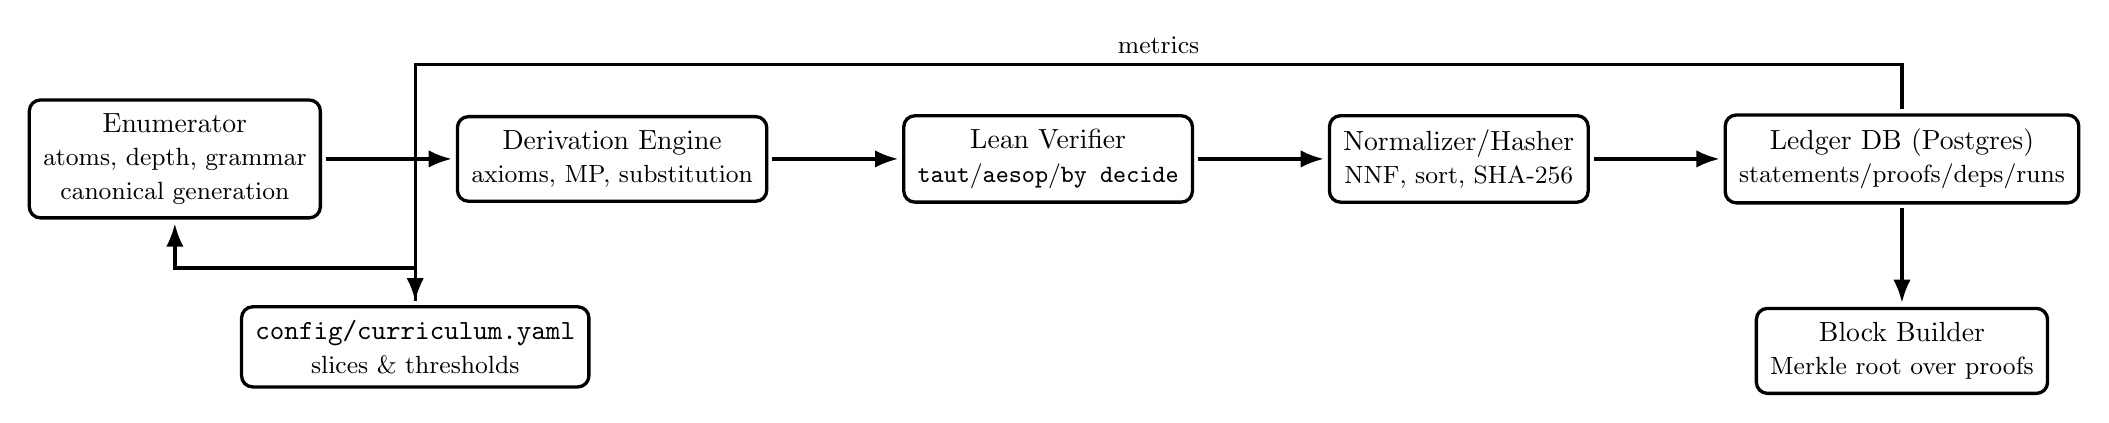
\begin{tikzpicture}[node distance=1.6cm and 1.6cm]
  \node[process] (enum) {Enumerator\\\small atoms, depth, grammar\\\small canonical generation};
  \node[process, right=of enum] (derive) {Derivation Engine\\\small axioms, MP, substitution};
  \node[process, right=of derive] (lean) {Lean Verifier\\\small \texttt{taut}/\texttt{aesop}/\texttt{by decide}};
  \node[process, right=of lean] (canon) {Normalizer/Hasher\\\small NNF, sort, SHA-256};
  \node[datastore, right=of canon] (db) {Ledger DB (Postgres)\\\small statements/proofs/deps/runs};
  \node[process, below=1.2cm of db] (blocks) {Block Builder\\\small Merkle root over proofs};

  \draw[line] (enum) -- (derive);
  \draw[line] (derive) -- (lean);
  \draw[line] (lean) -- (canon);
  \draw[line] (canon) -- (db);
  \draw[line] (db) -- (blocks);

  % Curriculum YAML feedback
  \node[process, below=1.2cm of derive, xshift=-2.5cm] (yaml) {\texttt{config/curriculum.yaml}\\\small slices \& thresholds};
  \draw[line] (yaml) -- ++(0,1.0) -| (enum.south);
  \draw[line] (db) |- ++(0,1.2) -| node[pos=0.25,above,sloped]{\small metrics} (yaml.north);
\end{tikzpicture}
\caption{End-to-end pipeline: generation, derivation, Lean verification, normalization, ingestion, and block sealing.}
\end{figure}

\subsection{Data Model}
\noindent The core schema tracks systems, normalized statements, proofs, dependencies, runs, and blocks. Each statement has a canonical hash computed from a normalized AST; each proof records method, prover, duration, status, and transcript hash. \emph{UPSERT} rules ensure idempotency and determinism.

\section{The Logic Ladder}
We climb theories via bounded \emph{slices}, saturating each before ratcheting difficulty:

\begin{figure}[!htbp]
\centering
\resizebox{!}{0.76\textheight}{%
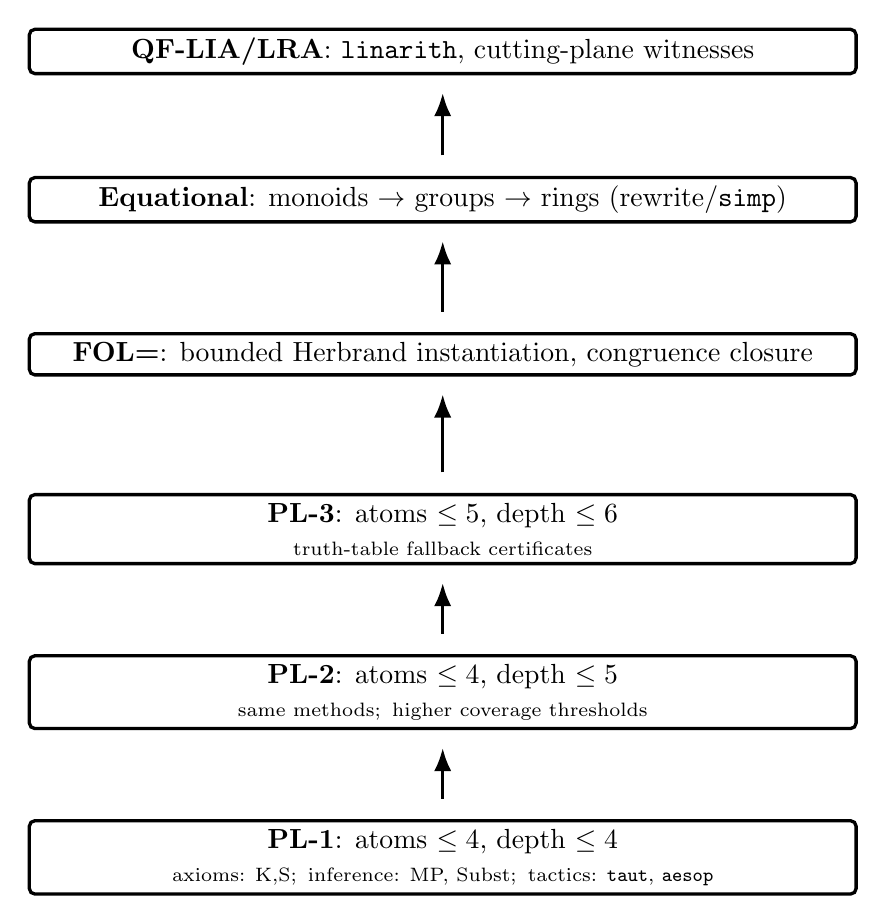
\begin{tikzpicture}[
    box/.style={block, minimum width=10.5cm, align=center},
    y=1.15cm
]

\node (pl1) [box] at (0,0)
{\textbf{PL-1}: atoms $\le 4$, depth $\le 4$\\
\scriptsize axioms: K,S;\, inference: MP, Subst;\, tactics: \texttt{taut}, \texttt{aesop}};

\node (pl2) [box, above=1.10cm of pl1]
{\textbf{PL-2}: atoms $\le 4$, depth $\le 5$\\
\scriptsize same methods;\, higher coverage thresholds};

\node (pl3) [box, above=1.10cm of pl2]
{\textbf{PL-3}: atoms $\le 5$, depth $\le 6$\\
\scriptsize truth-table fallback certificates};

\node (fol) [box, above=1.45cm of pl3]
{\textbf{FOL=}: bounded Herbrand instantiation, congruence closure};

\node (eq)  [box, above=1.35cm of fol]
{\textbf{Equational}: monoids $\to$ groups $\to$ rings (rewrite/\texttt{simp})};

\node (lia) [box, above=1.25cm of eq]
{\textbf{QF-LIA/LRA}: \texttt{linarith}, cutting-plane witnesses};

\foreach \lower/\upper in {pl1/pl2, pl2/pl3, pl3/fol, fol/eq, eq/lia}{
  \draw[-Latex, very thick,
        shorten >=6pt,
        shorten <=7pt] 
        (\lower.north) -- (\upper.south);
}

\end{tikzpicture}%
}
\caption{The curriculum ladder: each slice is saturated (coverage and success thresholds) before ratcheting.}
\label{fig:ladder}
\end{figure}

\section{Formalization of Ledger Semantics}
\begin{definition}[Canonical Identity]
Let $\mathcal{N}(s)$ be a normalization of formula $s$ (NNF, commutative sorting, right-association). The canonical identity is $\hash(s) \coloneqq \mathrm{SHA256}(\mathcal{E}(\mathcal{N}(s)))$, where $\mathcal{E}$ encodes the AST into bytes.
\end{definition}

\begin{definition}[Monotone Ledger]
A ledger $\ledger$ is a sequence of blocks $(B_1, B_2,\dots)$ where each $B_t$ is a finite set of proofs with (i) new statements by \hash, (ii) verified status in Lean, and (iii) a Merkle root $R_t$ computed over the sorted proof IDs. The ledger is \emph{monotone} if $\bigcup_{i\le t} B_i \subseteq \bigcup_{i\le t+1} B_i$ for all $t$.
\end{definition}

\begin{remark}[Determinism]
Given fixed slice parameters and toolchain versions, \system\ is deterministic: re-running a slice yields identical statements, proofs, and $R_t$.
\end{remark}

\section{Algorithms}
\subsection{Derivation Loop (PL)}
\begin{algorithm}[H]
\DontPrintSemicolon
\SetKwInOut{Input}{input}\SetKwInOut{Output}{output}
\Input{axioms $\mathcal{A}$ (K,S), known set $\mathcal{K}$, slice caps $(\text{atoms}, \text{depth}, \text{breadth}, \text{total})$}
\Output{new statements $\Delta \subseteq \mathcal{S}$ with proofs}
\BlankLine
\For{$\text{step}=1,2,\dots$}{
  $\mathcal{I}\leftarrow$ \emph{instantiate}(\,$\mathcal{A}$; atoms, depth\,)\;
  $\mathcal{C}\leftarrow \mathcal{K}\cup \mathcal{I}$\;
  $\Delta \leftarrow \{\,q \mid (p, p\to q)\subseteq \mathcal{C} \text{ (top-level MP), caps respected}\,\}$\;
  \For{$s\in \Delta$}{
     try Lean tactics with timeout; if fail and $s$ is tautology, use truth-table $\Rightarrow$ \texttt{by decide}\;
     persist $(s,\text{proof})$ if \hash\ unseen; update dependencies and block buffer\;
  }
  \If{caps exhausted or no new statements}{\textbf{break}}
}
\caption{Bounded-complete derivation in PL}
\end{algorithm}

\subsection{Normalization Highlights}
\begin{itemize}[leftmargin=1.5em]
  \item Right-associate implications: $a\to(b\to c) \leadsto a\to b\to c$; preserve explicit left parentheses (e.g.\ $(a\to b)\to c$).
  \item Sort commutative operands for $\land,\lor$; constant-fold trivialities; alpha-rename.
\end{itemize}

\section{Block Construction}
\begin{figure}[!htbp]
\centering
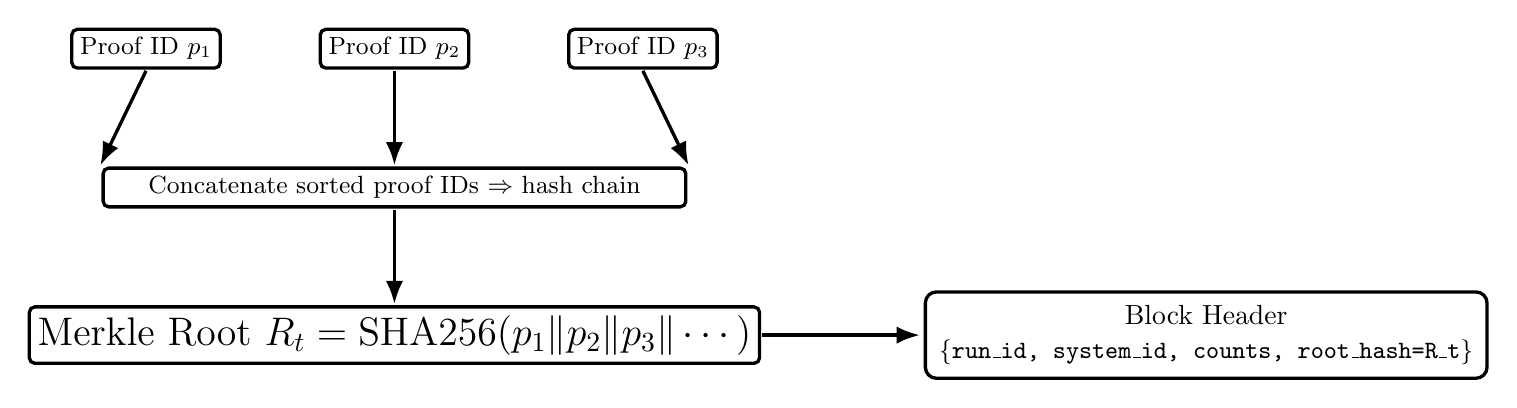
\begin{tikzpicture}
  \node[block] (p1) {\small Proof ID $p_1$};
  \node[block, right=1.2cm of p1] (p2) {\small Proof ID $p_2$};
  \node[block, right=1.2cm of p2] (p3) {\small Proof ID $p_3$};

  \node[block, below=1.2cm of p2, minimum width=7.4cm] (concat) {\small Concatenate sorted proof IDs $\Rightarrow$ hash chain};
  \draw[line] (p1.south) -- (concat.north west);
  \draw[line] (p2.south) -- (concat.north);
  \draw[line] (p3.south) -- (concat.north east);

  \node[block, below=1.2cm of concat] (root) {\Large Merkle Root $R_t=\mathrm{SHA256}(p_1 \| p_2 \| p_3 \|\cdots)$};
  \draw[line] (concat.south) -- (root.north);

  \node[process, right=2.0cm of root] (header) {Block Header\\\small \texttt{\{run\_id, system\_id, counts, root\_hash=R\_t\}}};
  \draw[line] (root.east) -- (header.west);
\end{tikzpicture}
\caption{Block sealing with a Merkle-style commitment over proof IDs.}
\label{fig:block-construction}
\end{figure}

\section{Interface: API, UI, and AI}
\paragraph{API.} Typed FastAPI endpoints: \path{/metrics}, \path{/theories}, \path{/blocks/latest?system=pl}, \path{/statements?hash=\dots}, \path{/lemmas/top}. Responses use Pydantic models for tool-calling reliability.

\paragraph{UI.} Two pages: \path{/ui} (dashboard with counters, depth histogram, recent statements) and \path{/ui/s/<hash>} (statement detail with proofs and DAG neighbors).

\paragraph{AI Wrapper.} A tool-calling model consumes the typed API: search, traverse, export, run bounded derivations. Human- and model-authored textbooks and papers hyperlink every claim to a ledger hash.

\subsubsection*{Abstention-First AI Wrapper}
Unless a query resolves to a canonical proof hash in the ledger, the wrapper returns \texttt{Unknown}. Proof-or-abstain aligns behavior with confidence targets and makes audit trivial.

\section{Evaluation \& Scaling Laws}
\paragraph{Metrics.} Proofs/sec, success rate, dedupe ratio, lemma reuse, depth coverage.

\begin{figure}[!htbp]
\centering
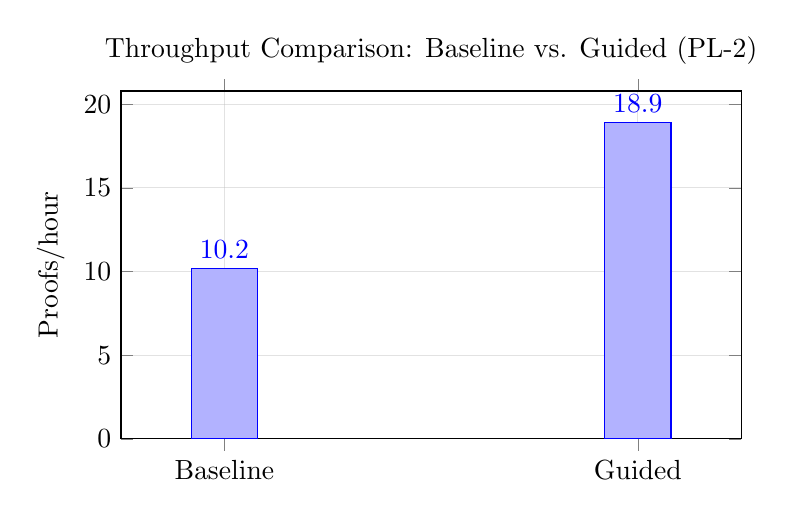
\begin{tikzpicture}
\begin{axis}[
  ybar, ymin=0, width=0.78\linewidth, height=6.0cm,
  bar width=24pt, ylabel={Proofs/hour},
  symbolic x coords={Baseline, Guided},
  xtick=data, nodes near coords,
  title={Throughput Comparison: Baseline vs. Guided (PL-2)},
  enlarge x limits=0.25, grid=both, grid style={faint}
]
\addplot coordinates {(Baseline,10.20) (Guided,18.90)};
\end{axis}
\end{tikzpicture}
\caption{A/B comparison of proof throughput at the PL-2 slice under identical budgets.
Guided policy achieved \textbf{+85.3\%} proofs/hour (see Appendix~A).}
\label{fig:pl2_bar}
\end{figure}

% ============================================================
% === NEW THEORY SECTIONS (inserted after prior §9.6) ========
% ============================================================

\section{Reflexive Formal Learning and the Physics of Self-Improvement}
\label{sec:rfl}
\textbf{Reflexive Formal Learning (RFL)} unifies generation, verification, and reflection into a single dynamical system. Let $\Pi_t$ denote the verifier ladder configuration at time $t$, $\mathcal{K}_t$ the ledger-saturated knowledge set, and $\mathcal{A}_t$ the abstention set harvested under budgets. An iteration is
\[
(\mathcal{K}_t, \Pi_t, \mathcal{A}_t)\;\xrightarrow{\;\text{policy}\;}\;(\mathcal{K}_{t+1}, \Pi_{t+1}),
\]
where $\mathcal{K}_{t+1} \supseteq \mathcal{K}_t$ by monotonicity, and $\Pi_{t+1}$ updates to reduce future abstentions under the same slice constraints.

\paragraph{Feedback triad.} Generate $\to$ Verify $\to$ Reflect (GVR) forms a closed loop, converting abstention mass into a \emph{learning signal}. The abstention distribution localizes epistemic entropy by depth, rule, and theory fragment; the policy learns to prioritize actions that minimize future abstention under fixed budgets.

\begin{figure}[!htbp]
\centering
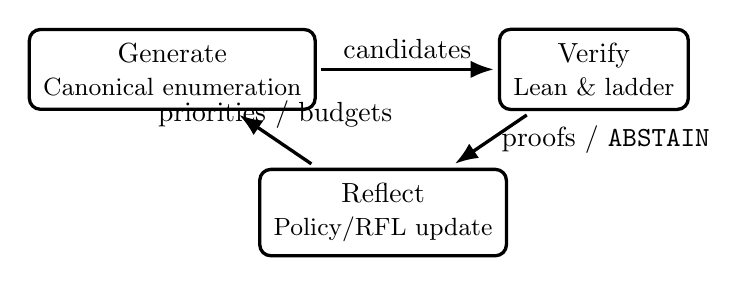
\begin{tikzpicture}[node distance=2.2cm]
  \node[process] (gen) {Generate\\\small Canonical enumeration};
  \node[process, right=of gen] (ver) {Verify\\\small Lean \& ladder};
  \node[process, below=1.2cm of $(gen)!0.5!(ver)$] (ref) {Reflect\\\small Policy/RFL update};

  \draw[line] (gen) -- node[midway,above]{candidates} (ver);
  \draw[line] (ver) -- node[midway,right]{proofs / \texttt{ABSTAIN}} (ref);
  \draw[line] (ref) -- node[midway,above]{priorities / budgets} (gen);
\end{tikzpicture}
\caption{Feedback triad (GVR): \emph{Reflexive Formal Learning}.}
\label{fig:feedback-triad}
\end{figure}

\paragraph{Physics analogy.} RFL is to cognition what gradient flow is to optimization: an invariant direction of improvement defined by verifiable work (accepted proofs) and measurable deficit (abstentions).

\section{Dual Attestation and the Chain of Verifiable Cognition}
\label{sec:dual-attest}
\textbf{Dual attestation} notarizes both the \emph{reasoning} and the \emph{interaction}. Let $R_t$ be the Merkle root over proof IDs in block $t$, and $U_t$ the Merkle root over user-interface inputs (queries, confirmations, corrections) within the same epoch. We define a composite epistemic root
\[
H_t \;=\; \mathrm{SHA256}(R_t \,\|\; U_t)
\]
binding what was \emph{thought} to what was \emph{asked/confirmed}. This braid yields the \emph{Chain of Verifiable Cognition}.

\begin{figure}[!htbp]
\centering
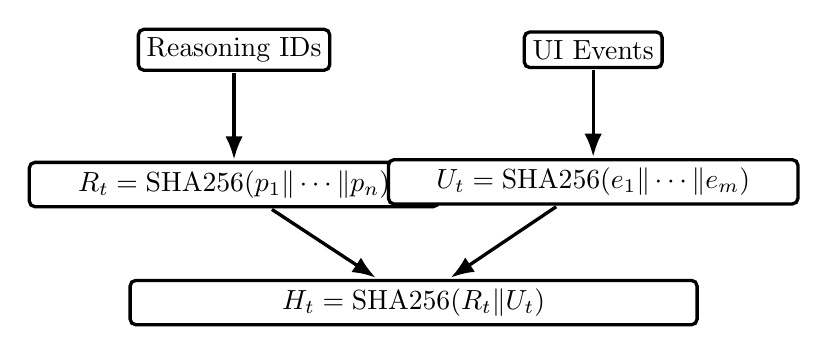
\begin{tikzpicture}[node distance=1.8cm]
  \node[block] (r1) {Reasoning IDs};
  \node[block, right=2.4cm of r1] (u1) {UI Events};
  \node[block, below=1.1cm of r1, minimum width=5.2cm] (rroot) {$R_t=\mathrm{SHA256}(p_1\|\cdots\|p_n)$};
  \node[block, below=1.1cm of u1, minimum width=5.2cm] (uroot) {$U_t=\mathrm{SHA256}(e_1\|\cdots\|e_m)$};
  \node[block, below=1.2cm of $(rroot)!0.5!(uroot)$, minimum width=7.2cm] (hroot) {$H_t=\mathrm{SHA256}(R_t\|U_t)$};

  \draw[line] (r1) -- (rroot);
  \draw[line] (u1) -- (uroot);
  \draw[line] (rroot) -- (hroot);
  \draw[line] (uroot) -- (hroot);
\end{tikzpicture}
\caption{Dual-Merkle attestation: UI-Merkle and Reasoning-Merkle braid into $H_t$.}
\label{fig:dual-merkle}
\end{figure}

\paragraph{Consequence.} Every claim can be audited against both \emph{how it was derived} and \emph{what the user believed or corrected}. This closes the last provenance gap for safety, compliance, and scientific reproducibility.

\section{User-Verified Input Loop and the Completion of Trust}
\label{sec:uvil}
The \textbf{User-Verified Input Loop (UVIL)} elevates user inputs to \emph{first-class epistemic objects}. Each input $e$ is normalized, optionally signed, and recorded into the UI-Merkle set. Corrections/abstentions become \emph{epistemic transactions}:
\[
\tau = \langle \texttt{actor},\ \texttt{kind}\in\{\text{confirm},\text{correct},\text{abstain}\},\ \texttt{target\_hash},\ \texttt{meta} \rangle.
\]
UVIL completes the trust circuit: human judgment and machine logic co-author the ledger with symmetric cryptographic guarantees. This generalizes to \emph{private truth ledgers} for legal and financial documents, where confidentiality-preserving commitments reference public headers.

\section{The Learning Law: A Symbolic Analogue to Gradient Descent}
\label{sec:learning-law}
We formalize a symbolic update law isomorphic to gradient-based learning. Let $\mathcal{U}_t(s)\in[0,1]$ denote the \emph{uncertainty} of statement schema $s$ estimated from abstention statistics and failed attempts at slice $t$. The RFL objective is to minimize expected uncertainty under budget $\mathcal{B}$ while preserving correctness:

\begin{theorem}[Symbolic Descent Step (informal)]
\label{thm:symbolic-descent}
Fix a slice and budget $\mathcal{B}$. A policy update that increases expected acceptance of candidates with $\mathcal{U}_t(s)>\tau$ and decreases mass on actions yielding repeated abstentions implements a descent step on the epistemic potential
\[
\Phi(\mathcal{K}_t) \;=\; \mathbb{E}_{s\sim\mathcal{D}_t}\,[\,\mathcal{U}_t(s)\,]
\]
subject to verification constraints. Consequently,
\[
\mathcal{K}_{t+1} \;=\; \mathcal{K}_t \;\cup\; \{\, s \mid \mathrm{provable}(s;\mathcal{B}) \wedge \mathcal{U}_t(s)>\tau \,\}
\]
\end{theorem}

\paragraph{RL isomorphism.} Treat verified acceptance as reward $r{=}1$, abstention as $r{=}0$, and false-accept as disallowed. The bandit objective maximizing $\mathbb{E}[r]$ under structural constraints (slice, budgets) is equivalent to minimizing $\Phi$. Policy gradients thus align with reductions in abstention mass, providing a mechanistic bridge to gradient descent/RL.

% ============================================================
% ================== RELATED WORK + POSITIONING ==============
% ============================================================

\section{Related Work and Differentiation}
Prior systems include:
\begin{itemize}[leftmargin=1.5em]
  \item \textbf{Mathlib (Lean):} extensive libraries; not a cryptographic ledger of growth.
  \item \textbf{Metamath/Isabelle/Coq:} proof assistants; lack dual attestation and curriculum-sliced data generation.
  \item \textbf{SMT/SAT toolchains:} produce witnesses; not a monotone, auditable knowledge substrate.
\end{itemize}
\system{} is novel in combining: (i) block-sealed monotonicity, (ii) authentic synthetic data generation, (iii) curriculum-based tractability, (iv) dual attestation (UI \& reasoning), and (v) RFL, a lawful path to self-improvement.

\section{Strategic Positioning}
\system{} is a \emph{substrate} rather than an application. It serves:
\begin{itemize}[leftmargin=1.5em]
  \item \textbf{Safety:} proof-or-abstain by construction; abstention telemetry for governance.
  \item \textbf{Capability:} compounding growth via RFL; improved search at fixed budgets.
  \item \textbf{Discovery:} a planetary corpus of verifiable statements with perfect provenance.
\end{itemize}
\textbf{Acquisition rationale.} The acquirer owns the unique, defensible source of infinite verified reasoning data and the protocol that elevates cognition to an auditable asset.

\section{Roadmap}
\begin{itemize}[leftmargin=1.5em]
  \item \textbf{PL (live):} bounded-complete derivations; nightly blocks; metrics and UI.
  \item \textbf{FOL= (next):} congruence closure, bounded instantiation; slice ratchet.
  \item \textbf{Equational:} rewrite proofs (\texttt{simp}, Knuth--Bendix); algebraic hierarchies.
  \item \textbf{QF-LIA/LRA:} \texttt{linarith}, certificates; linear identities and bounds.
  \item \textbf{Dual attestation:} productionize UI-Merkle; public headers/private payloads.
  \item \textbf{RFL law:} publish scaling curves of abstention mass $\downarrow$ vs.\ throughput $\uparrow$.
\end{itemize}

\section{Conclusion: Toward the Ledger of All Thought}
\label{sec:conclusion}
As Bitcoin became the ledger for value, \system{} becomes the ledger for \emph{valid thought}. Dual attestation binds what is perceived to what is proven; RFL supplies the physics of improvement; the curriculum ladder tames combinatorics. What emerges is a world-scale protocol for verifiable cognition. \textbf{To own \system{} is to own the root of verifiable intelligence.}

\section*{References}
% Minimal placeholder; replace with .bib in production
\begin{itemize}[leftmargin=1.5em]
  \item Kalai, A.~T., Nachum, O., Vempala, S., Zhang, E. (2025). \emph{Why Language Models Hallucinate}. arXiv:2509.04664.
  \item de Moura, L., Ullrich, S. (2021--2025). \emph{Lean 4}. \url{https://leanprover.github.io}
  \item Nipkow, T., Paulson, L.~C., Wenzel, M. (2002). \emph{Isabelle/HOL}. Springer.
  \item Gonthier, G. (2008). \emph{Formal proof—The four-color theorem}. Notices AMS.
\end{itemize}

% ===================== APPENDICES =====================
\appendix

\section*{Appendix A: Operational Vertical Slice}
\label{app:ops-vertical-slice}
\addcontentsline{toc}{section}{Appendix A: Operational Vertical Slice}
\paragraph{Core idea.}
A \emph{Vertical Slice} demonstrates end-to-end impact on \emph{Trust/Safety} and \emph{Capability/Performance}, converting the ledger from potential to realized value.

\subsection*{Prong 1: Trust Demonstration (Proof-or-Abstain)}
\textbf{Mechanism.} The wrapper enforces \emph{proof-or-abstain}. Query $\to$ hash lookup $\to$ cite block if found; else return \texttt{Unknown}. \\
\textbf{KPI.} Abstention precision $\approx 1.0$; zero false-accepts by design.

\subsection*{Prong 2: Capability Demonstration (Neuro-Symbolic)}
\textbf{Mechanism.} Symbolic generation $\to$ neural policy learning on sealed blocks $\to$ guided search. \\
\textbf{KPI.} $\ge$\,\textbf{+25\%} proofs/hour and $+1$ depth at PL-2 vs.\ baseline under identical budgets.

\subsection*{Execution Grid (72h)}
\begin{itemize}[leftmargin=1.5em]
  \item \textbf{T+0--24h:} \path{/statements} by \hash; smoke \& enqueue; nightly append.
  \item \textbf{T+24--48h:} policy reranker stub; export ladder metrics; build 3 trust prompts with Merkle citations.
  \item \textbf{T+48--72h:} PL-2 A/B; block proof pack v1; publish dashboard deltas.
\end{itemize}

\subsection*{Risk Register (Condensed)}
\noindent\small
\begin{center}
\renewcommand{\arraystretch}{1.15}
\begin{tabular}{@{}p{0.22\linewidth} p{0.34\linewidth} p{0.34\linewidth}@{}}
\toprule
\textbf{Trap} & \textbf{Primary Defense} & \textbf{Early Warnings} \\
\midrule
Scaling wall & Guided, bounded, deduped; portfolio search & Frontier size $\uparrow$, depth stalls \\
Verification bottleneck & Ladder + cache + slow-path & P95 verify latency $\uparrow$ \\
Replication risk & Semi-closed data moat & External requests beyond headers \\
\bottomrule
\end{tabular}
\end{center}

\subsection*{Ablation Snapshot (Guided vs Baseline at PL)}
\vspace{-0.5em}
\noindent\small
\begin{center}
\resizebox{\linewidth}{!} & \textbf{Block Root (short)} \\
G-1234 & 0xabc123 & PL-2 & 48.2 & 16 & 1,250 & 105.3 & 3.21 & 12.4\% & 0xdef456 \\
BL-5678 & 0xfed987 & PL-2 & 47.8 & 16 & 674 & 200.2 & 1.47 & 16.1\% & 0xcba321 \\
\midrule
\multicolumn{5}{@{}l}{\textbf{Delta (G vs BL) at PL-2}} & \textbf{+85.3\%} & \textbf{--47.4\%} & \textbf{+8.70} & \textbf{--3.7 pp} & \\
\bottomrule
\end{tabular}%
}
\end{center}

\section*{Appendix B: Verification Ladder (Pseudocode)}
\vspace{-0.5em}
\begin{algorithm}[H]
\DontPrintSemicolon
\SetAlgoLined
\SetKwInOut{Input}{input}\SetKwInOut{Output}{output}
\Input{statement $s$, budgets $\mathcal{B}=\{(A, t_A), (B, t_B), (SMT, t_S)\}$}
\Output{$\langle$verified, proof, meta$\rangle$ or \texttt{ABSTAIN}}
\BlankLine
\ForEach{$(T, t) \in \mathcal{B}$ in order}{
   $\langle ok, prf, meta \rangle \leftarrow \textsc{TryVerifier}(s, T, t)$\;
   \If{$ok$}{
     \Return $\langle \texttt{true}, prf, \{T, t\}\cup meta \rangle$\;
   }
}
\Return \texttt{ABSTAIN}\;
\caption{Verification Ladder with Budgets}
\end{algorithm}

% ============================================================
\end{document}